\chapter{Implementation}\label{chapter:Implementation}

In this chapter described several approaches to improve genetic solver to solve more complex problems.
To do this, a benchmark measurement was made.
In this section we concentrate on this problem:

\begin{itemize}
	\item variants: 10,
	\item requests: 15,
	\item depth: 2,
	\item resources: 5,
	\item timeout: 5 minutes.
\end{itemize}

Due to the problem, the basic version of the genetic solver could not solve this problem at all. We do all this work to, firstly, achieve valid results, and then get an optimal or near-optimal solution. 
All measurements here and later were done five times.


We mark basic~\footnote{As a basic version taked version from 24.09.2019, commit: \href{https://git-st.inf.tu-dresden.de/mquat/mquat2/commit/57845c126c30a1ea59cb35eb16af0bd37930dda9}{57845c126c30a1ea59cb35eb16af0bd37930dda9}} version of the genetic solver as \textbf{B} (Basic).


\begin{figure}[h]
	\centering
	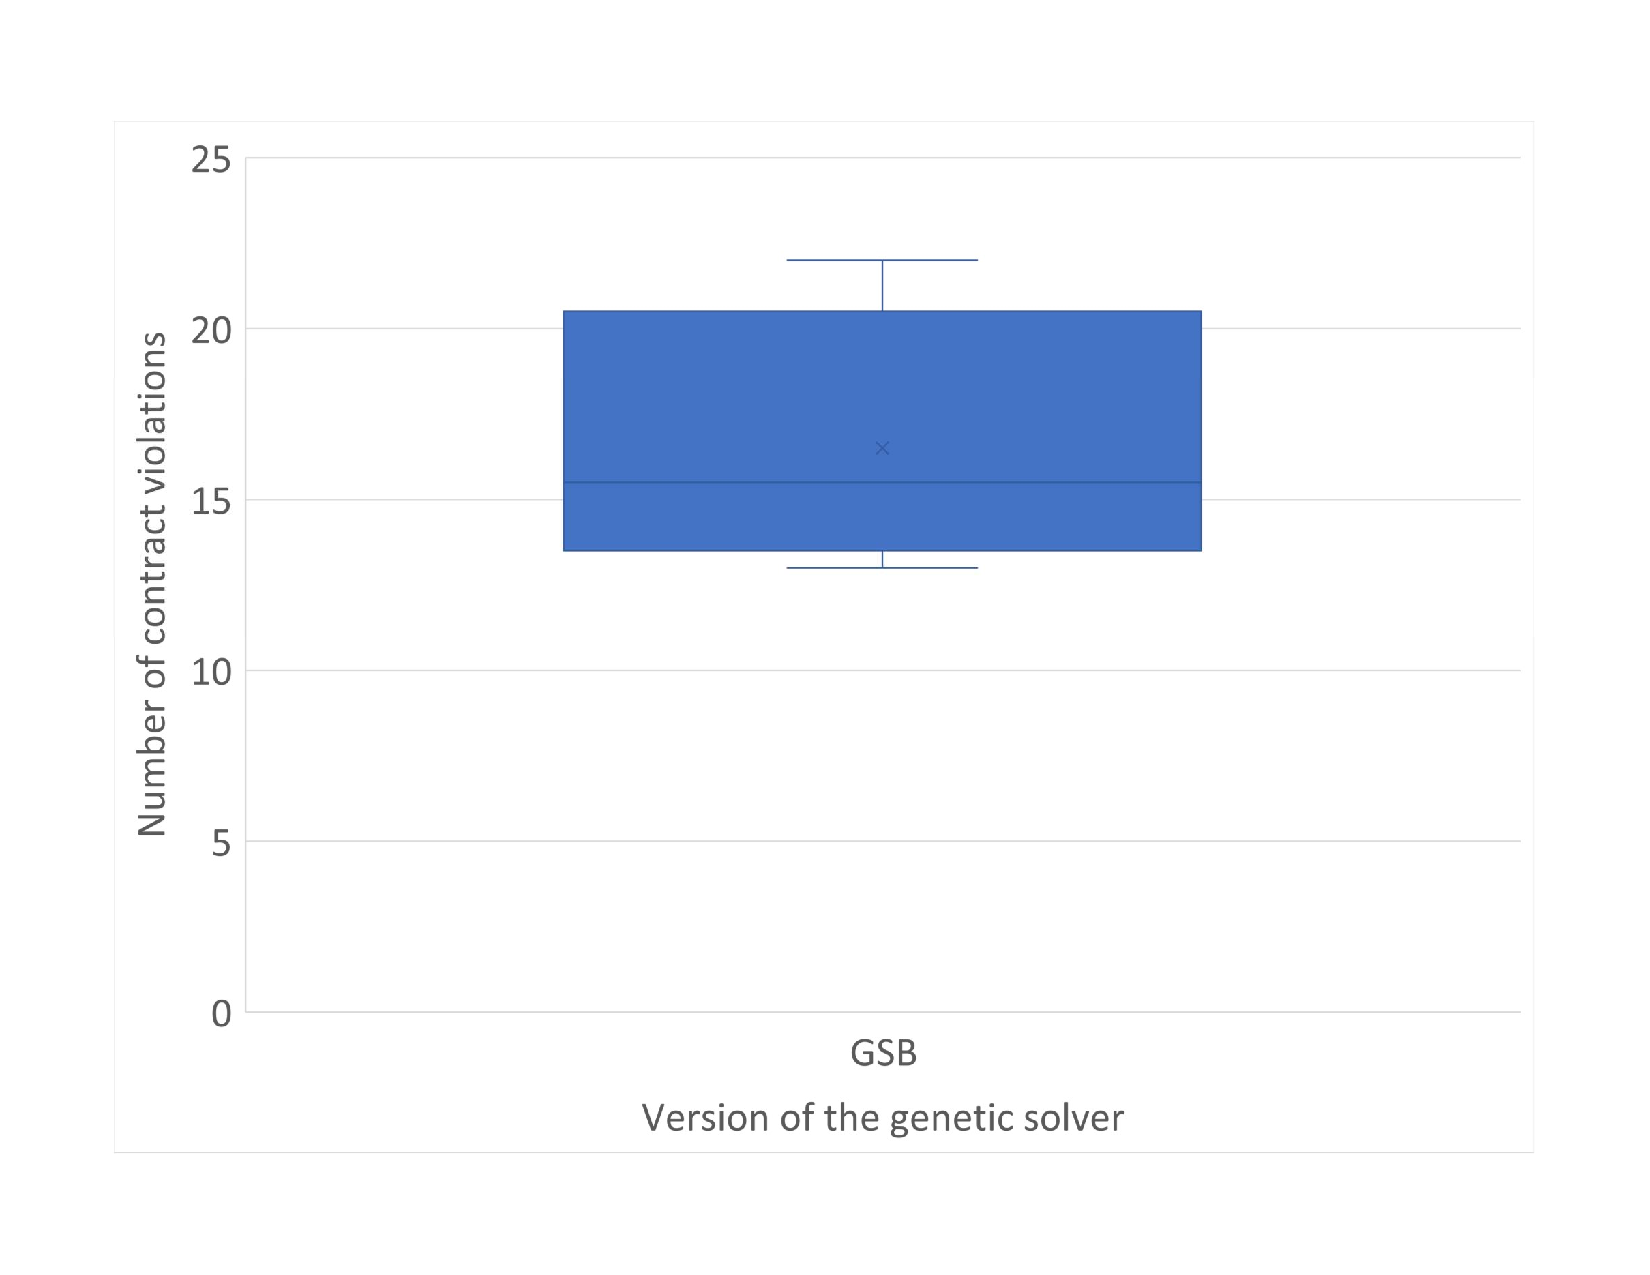
\includegraphics[width=\textwidth]{images/BoxPlotSolverBasic}
	\caption[Boxplot with a number of contract violations for the basic version of genetic solver]{}
	\label{fig:boxplotsolverbasic}
\end{figure}


Figure~\ref{fig:boxplotsolverbasic} shown the box-plot of number of contract violations in basic version of genetic solver. This plot shows, that \textbf{B} solver solve this task with number of contract violations in range from 13 to 22. As a result, there are no valid solutions for the current problem.




\section{Parameters that need tuning}

The first step to improve the genetic solver was a parameter optimization. To perform parameter optimization was performed a few important steps.

\begin{enumerate}
	\item Analysis of genetic solver to find out all parameters that could be changed externally. This parameters will be a hyperparameters that BRISE will tune.
	\item Adapt BRISE to work with the genetic solver.
	\item Prepare Experiment description for BRISE.
	\item Run BRISE to get the optimal configuration.
\end{enumerate}

Step 1 involves the analysis of the solver for the presence of parameters that can be changed externally. After deep-diving into the code of the genetic solver, the list of parameters was prepared:
	\paragraph{\texttt{selectorType}} - type of the selector algorithm that was mentioned in section~\ref{sec:GeneticAlgorithm:Selector}. It's a categorical parameter that has only two values (NSGA2 and SPEA2) due to technical limitation of used framework. Default value is \textit{NSGAII}.
	\paragraph{\texttt{Number of generation}} - number of generations that performed by the genetic solver, working as a termination condition, in this thesis we use only timeout termination, so this parameter set as a huge value,
	\paragraph{\texttt{PopulationSize}} - The parameter, that describes the number of individuals in a population. Default values is \textbf{500}, but for BRISE we decide to optimize this parameter in range from 100 to 5000.\\


Adaptation of the genetic solver to work in BRISE consists of preparing the executable file of the genetic solver and implementing a method for the worker component, which calls the executable file and returns the results with a number of contract violations and energy consumption.

Step number 3 means, that a user creates the experiment description file. This file describes parameters that need to optimize and BRISE components, such as selector, repeater, model and stop condition. The description of the parameters consists of a list of parameters. Each element of this list describes one hyperparameter that will be optimized. Each hyperparameter is described by a name, a range of values, or a set of values, the default value.

For parameter tuning of the genetic solver, we use Sobol sampling as a selector algorithm to get the new configuration of hyperparameters, student repeater with a minimal number of measurements - 3 and max number - 6. BRISE uses Bayesian Optimization (BO) as a prediction model.
To stop BRISE, we use a combination of time-based stop condition with timeout - 12 hours and guarantee stop condition, which guarantees a better result than a result with the default set of parameters. Experiment description file presented in appendix\todoR{ref to appendix with experiment description}.

Due to the technics of getting the default value of parameters described in Section~\ref{sec:Parameter Tuning Strategies}, we use values that used in the \textbf{B} version of the genetic solver. The main reason for this that BRISE uses a guarantee stop condition. Furthermore, values in the \textbf{B} solver were achieved empirically by developers. The default values are presented in Table~\ref{tab:Parameters_B-T}. Also, there are a few parameters that have a hard-coded value, and we do not tune them. We will discuss them in the next section, but their names and values also presented in Table~\ref{tab:Parameters_B-T}. These parameters have a gray color fill. 

We mark current version~\footnote{commit: \href{https://git-st.inf.tu-dresden.de/mquat/mquat2/commit/e103f52b3333900d61c6218a1f2ca811bca10289}{e103f52b3333900d61c6218a1f2ca811bca10289}} of the genetic solver as \textbf{B-T}(Basic-Tuned).


\begin{table}
	\centering
	\caption{Parameters of B and B-T versions of the genetic solver}\label{tab:Parameters_B-T}
	\resizebox{\textwidth}{!}{
		\begin{tabular}{c c c a a a a a a a a a a}
			\hline
			\rotatebox{90}{Genetic solver} & \rotatebox{90}{\texttt{selectorType}} & \rotatebox{90}{\texttt{PopulationSize}} & \rotatebox{90}{\texttt{lambda}} & \rotatebox{90}{\texttt{CrossoverRate}} & \rotatebox{90}{\texttt{mu}} & \rotatebox{90}{\texttt{MutationRate}} & \rotatebox{90}{\texttt{ResourceMutationProbability}}  & \rotatebox{90}{\texttt{CrossoverProbability}}  & \rotatebox{90}{\texttt{ValidityWeight}} & \rotatebox{90}{\texttt{SoftwareValidityWeight}} & \rotatebox{90}{\texttt{RandomSoftwareAssignmentAttempts}} & \rotatebox{90}{\texttt{populateSoftwareSolutionAttempts}} \\
			\hline			
			B & NSGA2 & 500 & 0.1 & 0.95 & 0.1 & 0.45 & 0.5 & 0.8 & 0.5 & 0.5 & 50 & 100 \\
			B-T & NSGA2 & 1533 & 0.1 & 0.95 & 0.1 & 0.45 & 0.5 & 0.8 & 0.5 & 0.5 & 50 & 100 \\
			\hline
		\end{tabular}
	}
\end{table}

The optimal configuration of parameters found by the BRISE is presented in the Table~\ref{tab:Parameters_B-T}.

\begin{figure}
	\centering
	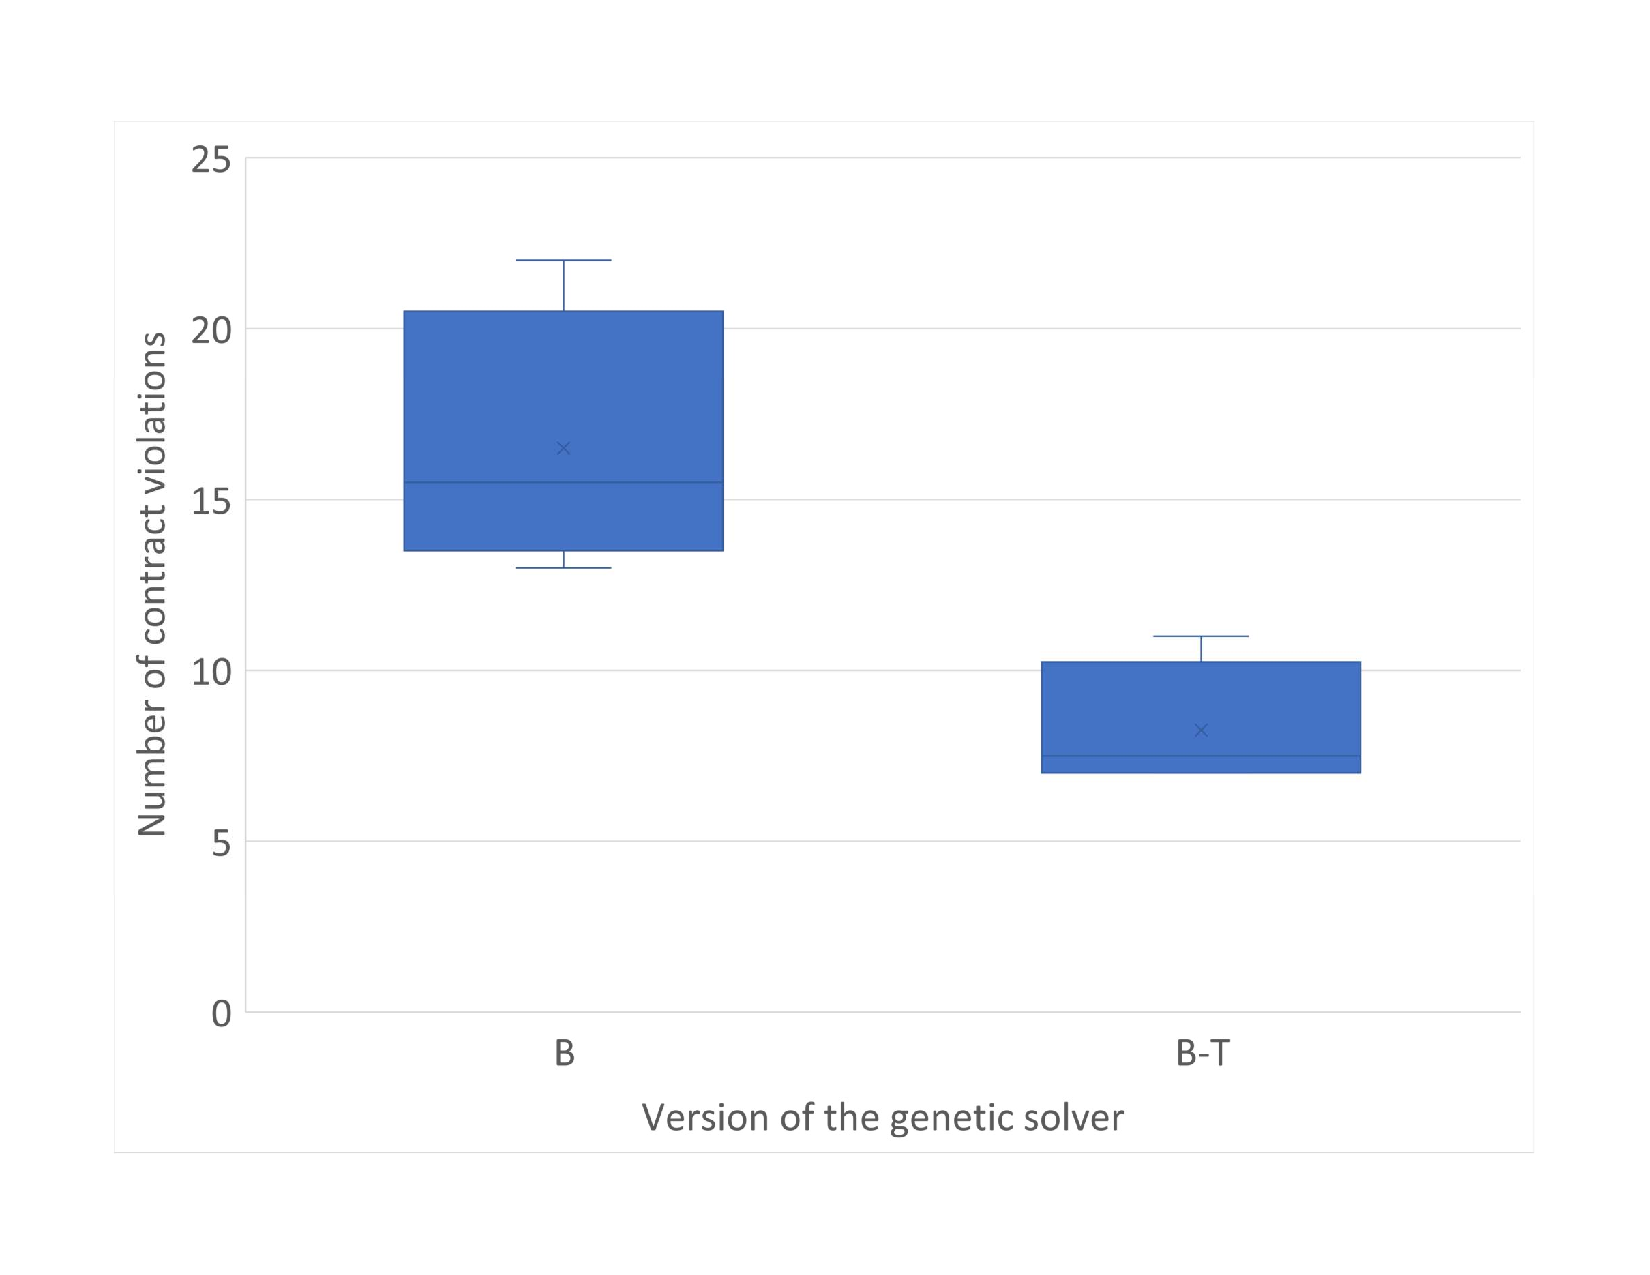
\includegraphics[width=\textwidth]{images/BoxPlotSolverBasicTuning}
	\caption[Boxplot with a number of contract violations for the basic version of genetic solver and with tuned parameters]{}
	\label{fig:boxplotsolverbasictuning}
\end{figure}

The results of solving the earlier described problem as a boxplot showed in Figure~\ref{fig:boxplotsolverbasictuning}. In the Figure~\ref{fig:boxplotsolverbasictuning} also showed the comparison between B and B-T versions.  The B version of the genetic solver with an optimized set of parameters gives a better result compared with the \textbf{B} version.

The max number of contract violations in the B-T version is 11 vise versa 22 in the B version. That shows that even the worsted result of B-T is better than the best result from the B version. The minimal number of contract violations in the B-T version is seven vise versa 13 in the B version. It is almost two times fewer contract violations. 

Received results answer the \textbf{RQ1}. Parameter tuning improves results, and it has a positive effect on the genetic solver, but results are still not valid. 

\section{More parameters}

In previous section we showed that not all parameters of the genetic solver exposed for external tuning. To make them changeable externally, we use \texttt{GoogleGuiceDependencyInjection}\footnote{\url{https://github.com/google/guice}} to change the values of these parameters during the solver call. Let us discuss this parameters:
	 \paragraph{\texttt{lambda}} - as mentioned in section~\ref{sec:GeneticAlgorithm:Selecto}, it describes the number of new offspring per generation. We use this parameter as a part of the population size.
	 The default value is 0.1 and the range of optimization from 0.0 to 1.0.
	 \paragraph{\texttt{CrossoverRate}} - as mentioned in section~\ref{sec:GeneticAlgorithmCrossover}, it describes the probability of two individuals to exchange their genes. The default value is 0.95. This is the default value for the crossover rate chosen by the developers of the Opt4J framework. BRISE will tune this parameter in range from 0.0 to 1.0.
	 \paragraph{\texttt{mu}} - as mentioned in section~\ref{sec:GeneticAlgorithm:Selector}, it describes the number of parents, selected by the selector to create new individuals. We use this parameter as a part of the population size.
	 The default value is 0.1 and the range of optimization from 0.0 to 1.0.
	 \paragraph{\texttt{MutationRate}} - as mentioned in section~\ref{sec:GeneticAlgorithmMutation}, it describes the probability of the individual to mutate. BRISE will tune this parameter in value range from 0.0 to 1.0 with default value 0.45 from the B version of the genetic solver.
	 \paragraph{\texttt{ResourceMutationProbability}} - the likelihood that during the mutation, the assigned resource will mutate. BRISE will tune this parameter in value range from 0.0 to 1.0 with default value 0.5 from the B version of the genetic solver.
	 \paragraph{\texttt{CrossoverProbability}} - it describes the probability of doing crossover that checks in the crossover operator. The default value of this parameter is 0.8. BRISE tune it in a range from 0.0 to 1.0. This parameter was removed in later versions of the genetic solver because it duplicates the functionality of \texttt{CrossoverRate}. This fact gives the answer on \textbf{RQ1}. It is one bad design choice that we want to find, according to \textbf{RQ2}.\\ 
	 

Within the genetic solver evaluator, two factors reduce the quality of the solution in the event of a contract breach or errors in dependencies in the software tree. These coefficients were not set for external tuning.
	 \paragraph{\texttt{ValidityWeight}} - coefficient that shows how each contract violation decreases  the quality of the solution.
	 \paragraph{\texttt{SoftwareValidityWeight}} - coefficient that shows how each error in software tree decrease the quality of the solution.\\

The default value for both parameters is 0.5. BRISE tune them in a range from 0.0 to 1.0.
	 
As described in Section~\ref{sec:GeneticSolver}, a creator creates random individuals for the initial population.
This method has two features that are necessary to obtain better individuals at the initial stage. These features have parameters:
	 \paragraph{\texttt{RandomSoftwareAssignmentAttempts}} - max number of attempts to set a valid software tree to the individual on the creation phase. The default value is 50.
	 \paragraph{\texttt{populateSoftwareSolutionAttempts}} -  max number of attempts to assign software components and resources to get a valid individual on the creation phase. The default value is 100.\\

BRISE tune both parameters in a range from 1 to 1000.

We mark current version~\footnote{commit: \href{https://git-st.inf.tu-dresden.de/mquat/mquat2/commit/e1db4a941622f9a6609ffcfb5d05df9e7abaffc2}{e1db4a941622f9a6609ffcfb5d05df9e7abaffc2}} of the genetic solver as \textbf{WHC-T}(Without Hard-Code-Tuned).

After optimization, we use optimized set of values of hyperparameters from BRISE, showed in Table~\ref{tab:Parameters_NHC-T}, as a parameters for the genetic solver. 

\begin{table}
	\centering
	\caption{Parameters of WHC-T version of the genetic solver}\label{tab:Parameters_NHC-T}
	\resizebox{\textwidth}{!}{
		\begin{tabular}{c c c c c c c c c c c c c}
			\hline
			\rotatebox{90}{Genetic solver} & \rotatebox{90}{\texttt{selectorType}} & \rotatebox{90}{\texttt{PopulationSize}} & \rotatebox{90}{\texttt{lambda}} & \rotatebox{90}{\texttt{CrossoverRate}} & \rotatebox{90}{\texttt{mu}} & \rotatebox{90}{\texttt{MutationRate}} & \rotatebox{90}{\texttt{ResourceMutationProbability}}  & \rotatebox{90}{\texttt{CrossoverProbability}}  & \rotatebox{90}{\texttt{ValidityWeight}} & \rotatebox{90}{\texttt{SoftwareValidityWeight}} & \rotatebox{90}{\texttt{RandomSoftwareAssignmentAttempts}} & \rotatebox{90}{\texttt{populateSoftwareSolutionAttempts}} \\
			\hline			
			WHC-T & SPEA2 & 2014 & 0.98 & 0.95 & 0.58 & 0.02 & 0.64 & 0.3 & 0.95 & 0.17 & 79 & 266 \\
			\hline
		\end{tabular}
	}
\end{table}

Results of the WHC-T version of the genetic solver presented as boxplot in comparison with earlier versions showed in Figure~\ref{fig:boxplotsolverNoHardcodedTuning}. This boxplot shows that the WHC-T version of the genetic solver is better in comparison to B-T. The max number of contract violations in WHC-T is \textbf{seven}. This number is equal to a minimum number of contract violations from the B-T version. The minimal number of violations is \textbf{three}, which means that solutions are still \textbf{not valid} for the current problem. 

\begin{figure}
	\centering
	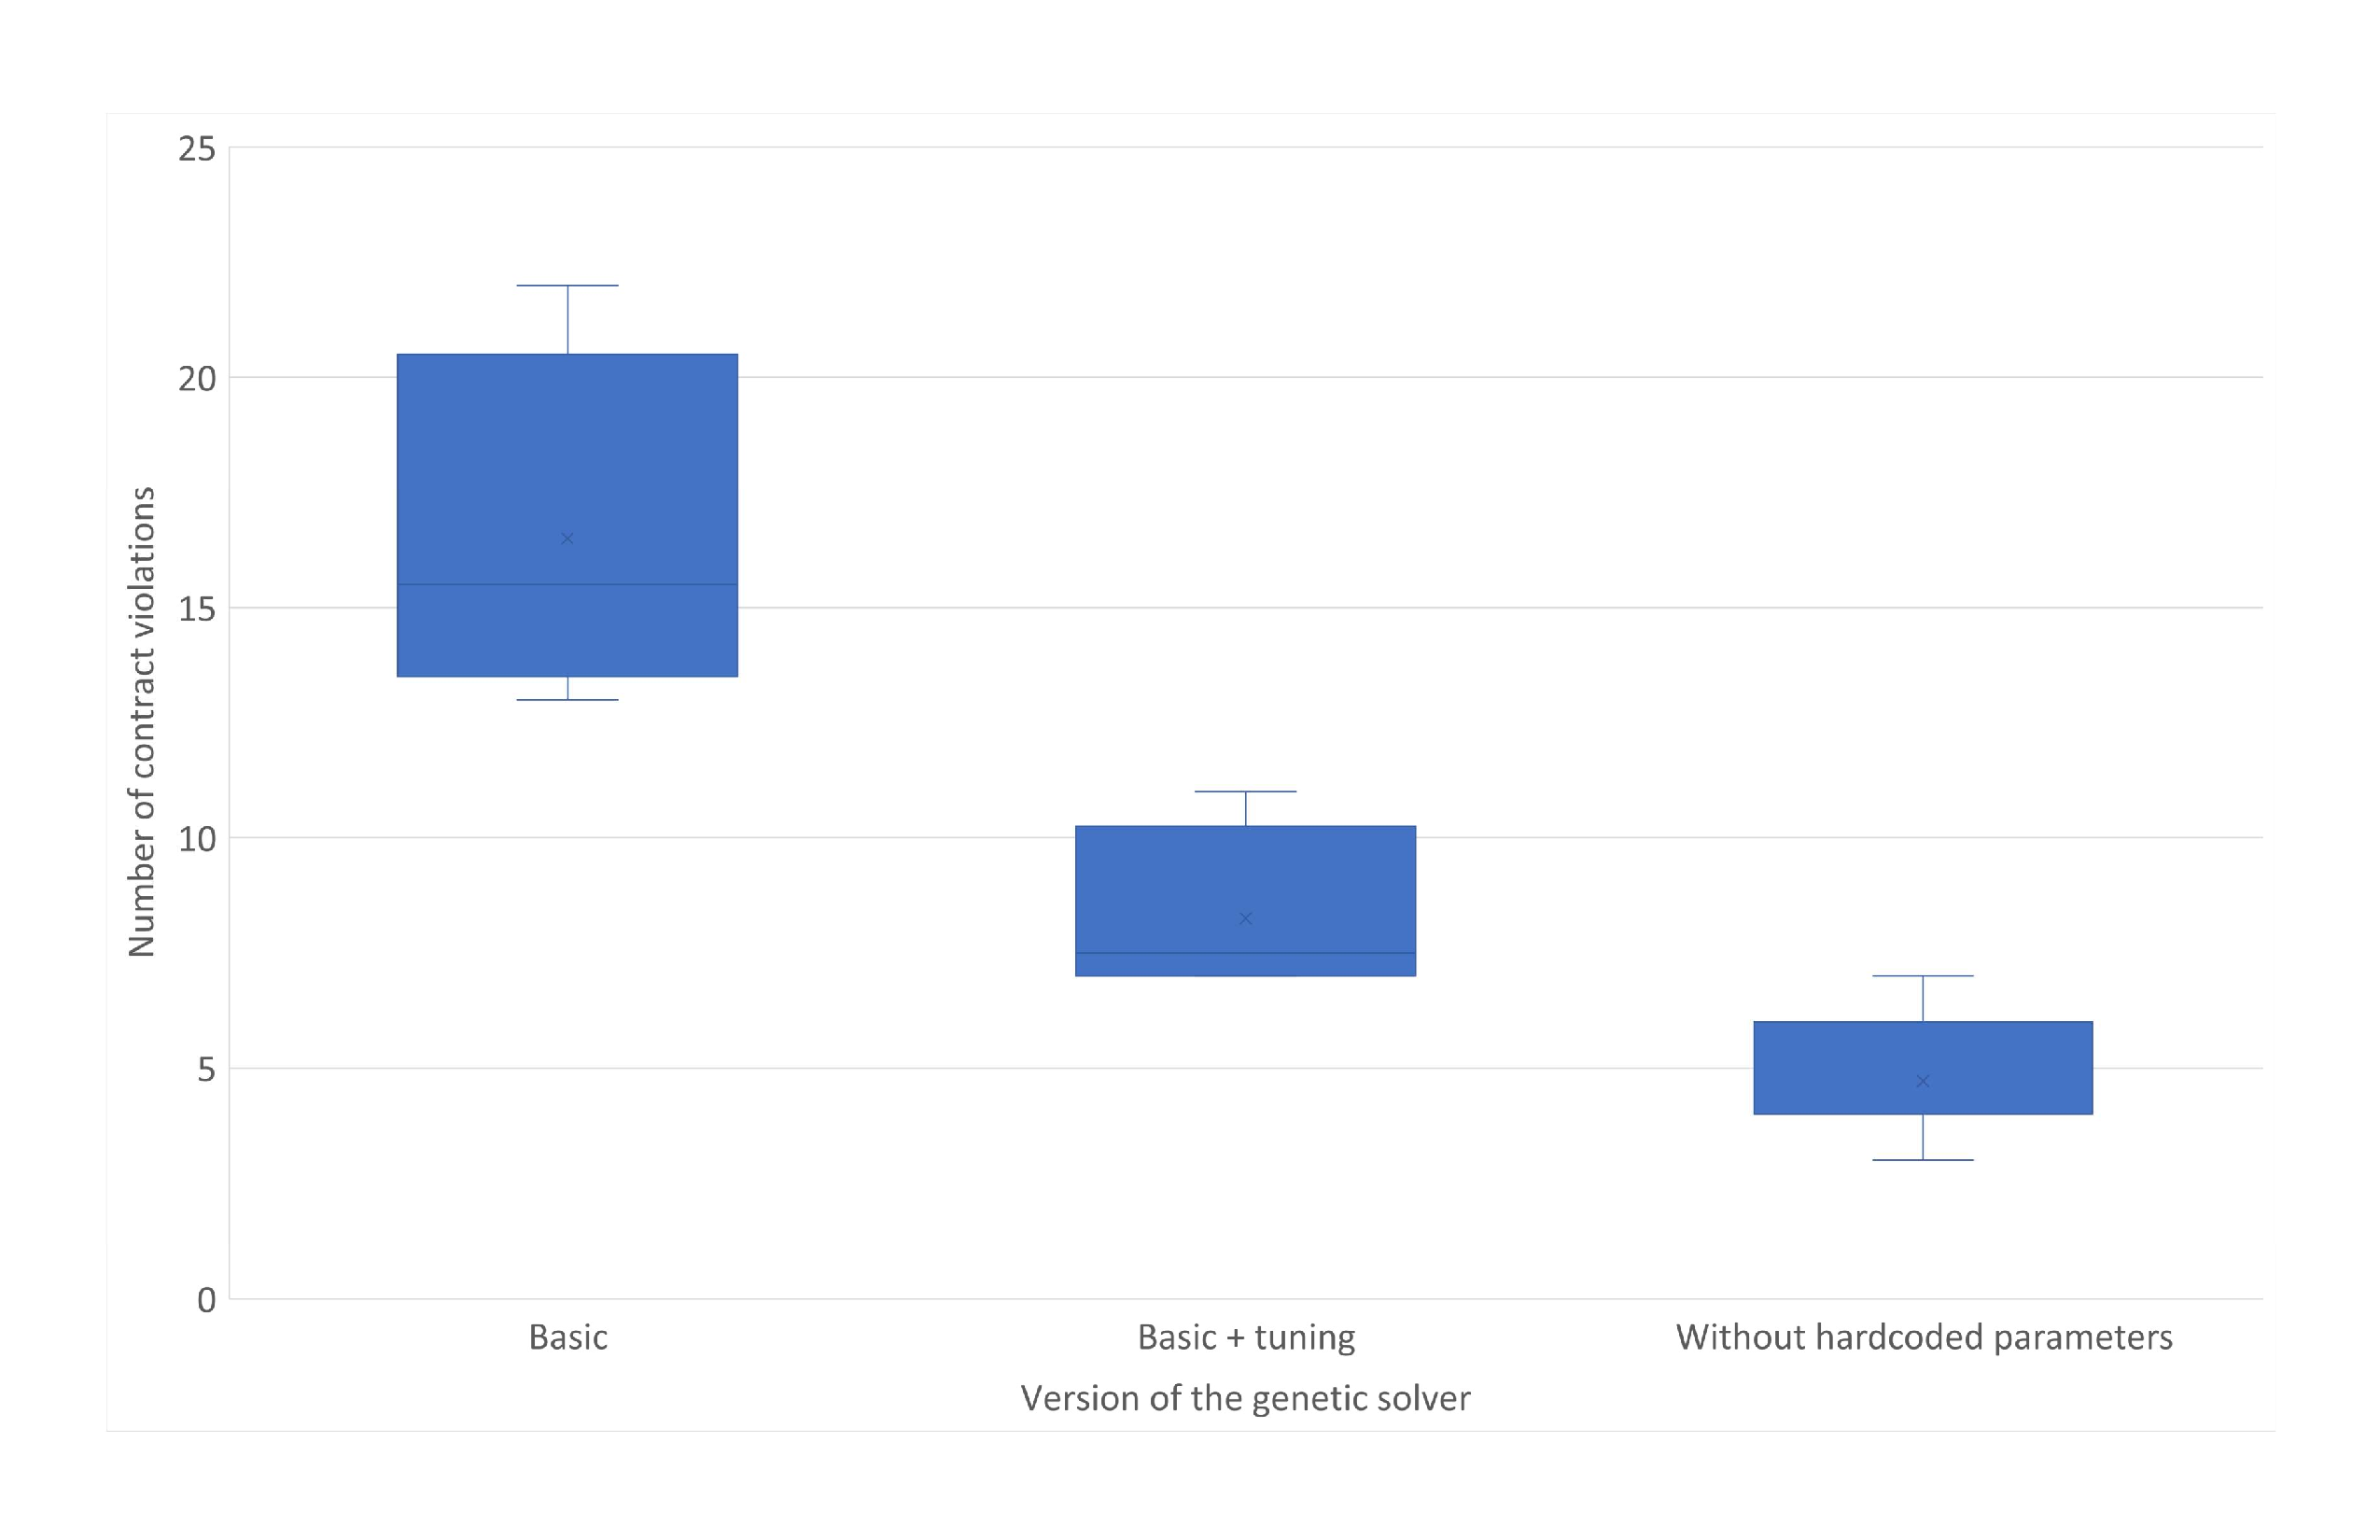
\includegraphics[width=\textwidth]{images/BoxPlotSolverNoHardcodedTuning.pdf}
	\caption[Boxplot with a number of contract violations for the genetic solver without hardcoded parameters in comparison with previous versions]{Boxplot with a number of contract violations for the genetic solver without hardcoded parameters in comparison with previous versions}
	\label{fig:boxplotsolverNoHardcodedTuning}
\end{figure}

This section shows how correctly selected parameter values affect the result of the algorithm. For the described problem without complex changes in the algorithm, we got a result that, in the worst-case, gave a solution that is almost twice as good as the best solution in the B version of the genetic solver. However, parameter optimization is not enough to obtain valid solutions for the tasks described at the beginning of this chapter. 

\section{Even more parameters}\label{sec:NP}

Since parameter tuning from the previous steps could not give valid results, we decide to use another approach called parameter engineering.
Detailed analysis of crossover and mutation operators showed that crossover point and mutation points are coarse-grained. The principle how these points defines described in Section~\ref{sec:GeneticAlgorithmCrossover} and Section~\ref{sec:GeneticAlgorithmMutation}.

We add a few more probabilities to crossover and mutation operators. These probabilities allow changing the location of crossover/mutation points in different ways of the Tree Shape Genotype.
There are:
	\paragraph{\texttt{CrossoverOnRandomChildProbability}} - the chance that crossover will occur on the random child or both children otherwise.
	\paragraph{\texttt{CrossoverOnRandomLevelProbability}} - the probability that describes a chance to do a crossover on random level of the tree, 
	\paragraph{\texttt{CrossoverOnRandomRequestProbability}} - the chance to do a crossover on random request,
	\paragraph{\texttt{MutationOnRandomChildProbability}} - the probability that describes a chance of mutation on a random child,
	\paragraph{\texttt{MutationOnRandomLevelProbability}} - the chance of mutation on a random level of the tree shape genotype.
	
The default value for there probabilities, except \texttt{CrossoverOnRandomRequestProbability}, is 0.5. For the \texttt{CrossoverOnRandomRequestProbability} is 0.0. These values we received empirically during developing.

This version~\footnote{commit: \href{https://git-st.inf.tu-dresden.de/mquat/mquat2/commit/817f7f1ef06f3acbbb4d5e24e32a26c5e6abc4b5}{817f7f1ef06f3acbbb4d5e24e32a26c5e6abc4b5}} of the genetic solver marked as \textbf{NP}(New Probabilities).

The set of parameters used during development is presented in Table~\ref{tab:Parameters_NP-T}. New parameters have the values described above. Furthermore, previously discussed parameters have values from the B version of the genetic solver. That means that all parameters are not tuned.

\begin{table}
	\centering
	\caption{Parameters of NP and NP-T versions of the genetic solver}\label{tab:Parameters_NP-T}
	\resizebox{\textwidth}{!}{
		\begin{tabular}{c c c c c c c c c c c c c c c c c}
			\hline
			\rotatebox{90}{Genetic solver} & 
			\rotatebox{90}{\texttt{selectorType}} & \rotatebox{90}{\texttt{PopulationSize}} & 
			\rotatebox{90}{\texttt{lambda}} & 
			\rotatebox{90}{\texttt{CrossoverRate}} & 
			\rotatebox{90}{\texttt{mu}} & 
			\rotatebox{90}{\texttt{MutationRate}} & \rotatebox{90}{\texttt{ResourceMutationProbability}}  &
			\rotatebox{90}{\texttt{ValidityWeight}} & \rotatebox{90}{\texttt{SoftwareValidityWeight}} & \rotatebox{90}{\texttt{RandomSoftwareAssignmentAttempts}} & \rotatebox{90}{\texttt{populateSoftwareSolutionAttempts}} &
			\rotatebox{90}{\texttt{CrossoverOnRandomChildProbability}} &
			\rotatebox{90}{\texttt{CrossoverOnRandomLevelProbability}} &
			\rotatebox{90}{\texttt{CrossoverOnRandomRequestProbability}} &
			\rotatebox{90}{\texttt{MutationOnRandomChildProbability}} &
			\rotatebox{90}{\texttt{MutationOnRandomLevelProbability}} \\
			\hline			
			NP & NSGA2 & 500 & 0.1 & 0.95 & 0.1 & 0.45 & 0.5 & 0.5 & 0.5 & 50 & 100 & 0.5 & 0.5 & 0.0 & 0.5 & 0.5 \\
			NP-T & NSGA2 & 2550 & 0.5 & 0.5 & 0.5 & 0.5 & 0.5 & 0.5 & 0.5 & 500 & 500 & 0.5 & 0.5 & 0.5 & 0.5 & 0.5 \\
			\hline
		\end{tabular}
	}
\end{table}

The result of the NP version of the genetic solver presented as boxplot in comparison with earlier versions showed in Figure~\ref{fig:boxplotsolverNewParameters}. If we compare the B and the NP versions, then both versions have non-optimized parameter values. The NP version has a minimal number if contract violations equal 3. It is three times fewer violations than in the best case if the B version. Moreover, this version of the genetic solver has results comparable to the results after parameter tuning in the WHC-T version. As a result, better-designed parameters could also improve the target system. 

\begin{figure}
	\centering
	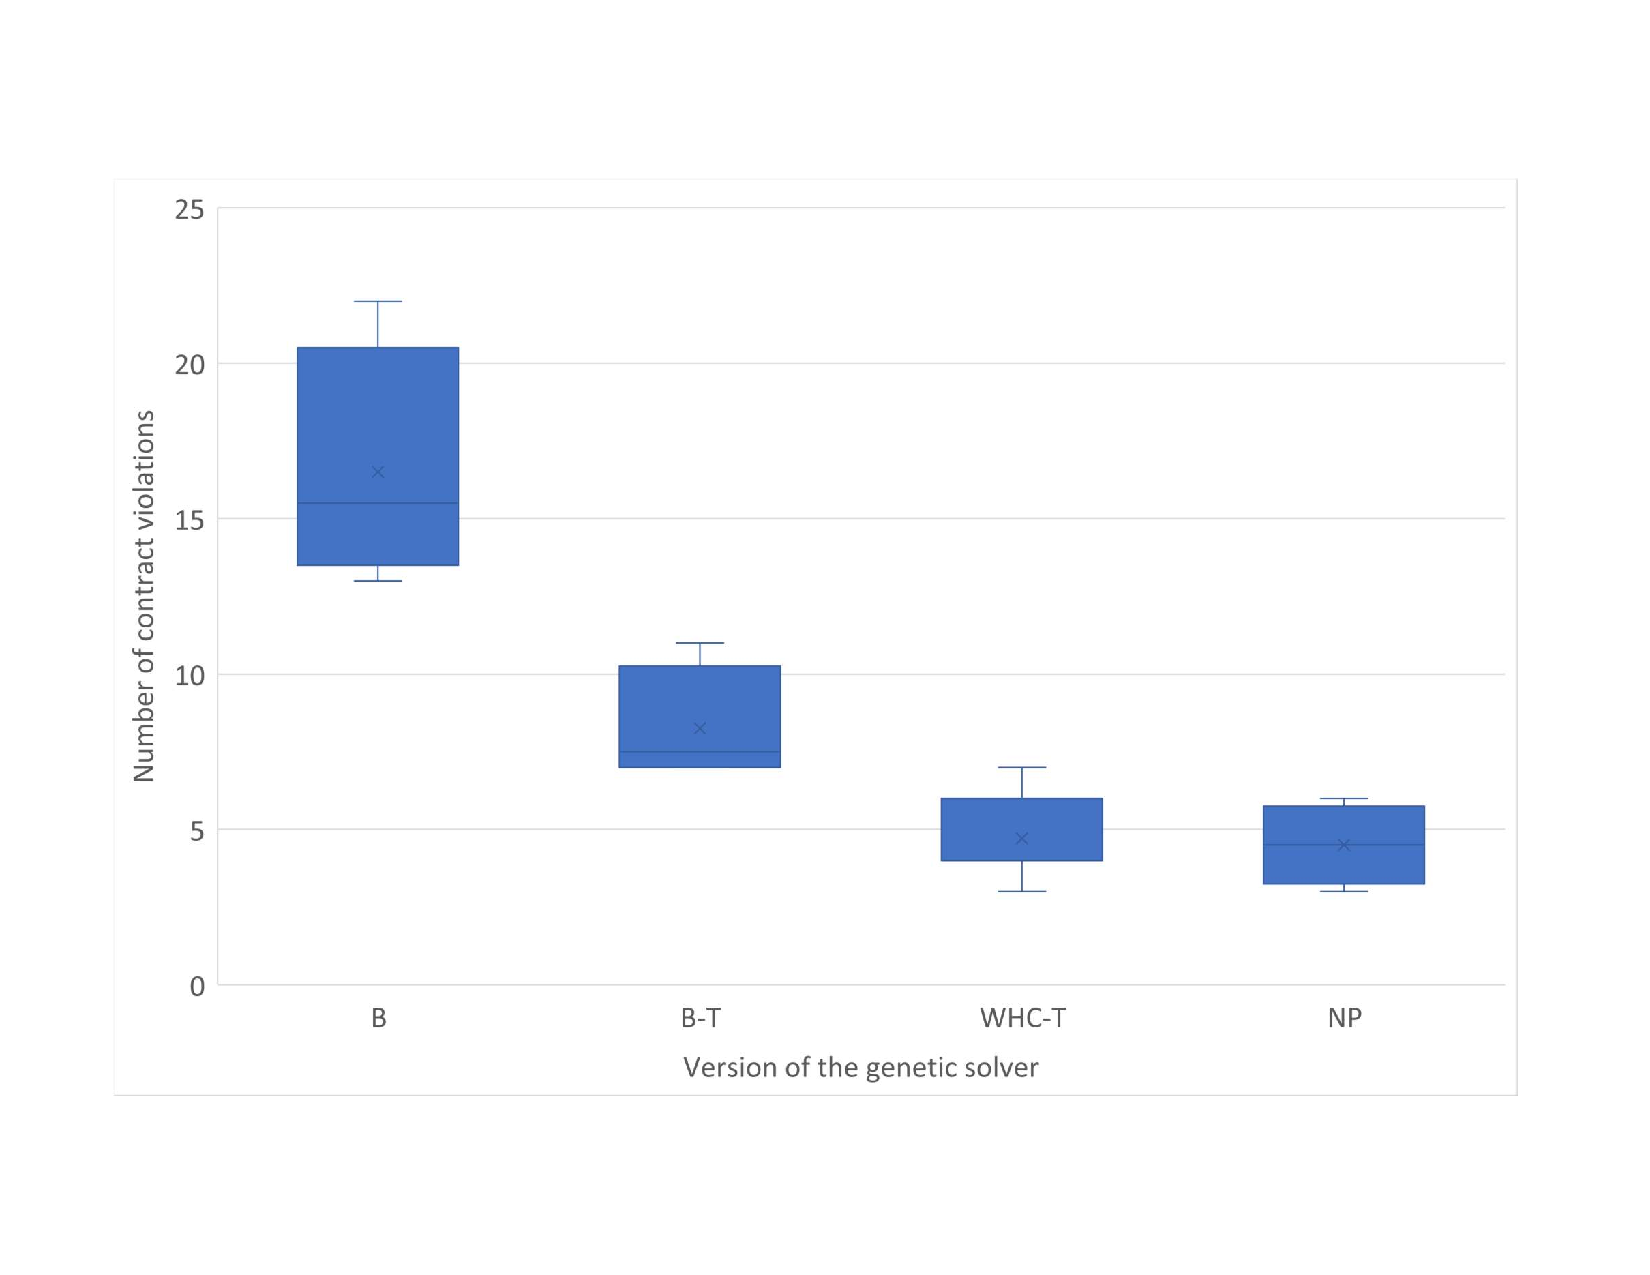
\includegraphics[width=\textwidth]{images/BoxPlotSolverNewParameters.pdf}
	\caption[Boxplot with a number of contract violations for the genetic solver with added probabilities without tuning in comparison with previous versions]{Boxplot with a number of contract violations for the genetic solver with added probabilities without tuning in comparison with previous versions}
	\label{fig:boxplotsolverNewParameters}
\end{figure}

After adding new parameters, we started BRISE to optimize all parameters. The optimized set of parameters presented in Table~\ref{tab:Parameters_NP-T}. We marked the NP version with optimized set of parameters as \textbf{NP-T}(New Probabilities-Tuned)~\footnote{commit: \href{https://git-st.inf.tu-dresden.de/mquat/mquat2/commit/e103f52b3333900d61c6218a1f2ca811bca10289}{e103f52b3333900d61c6218a1f2ca811bca10289}}.

\begin{figure}
	\centering
	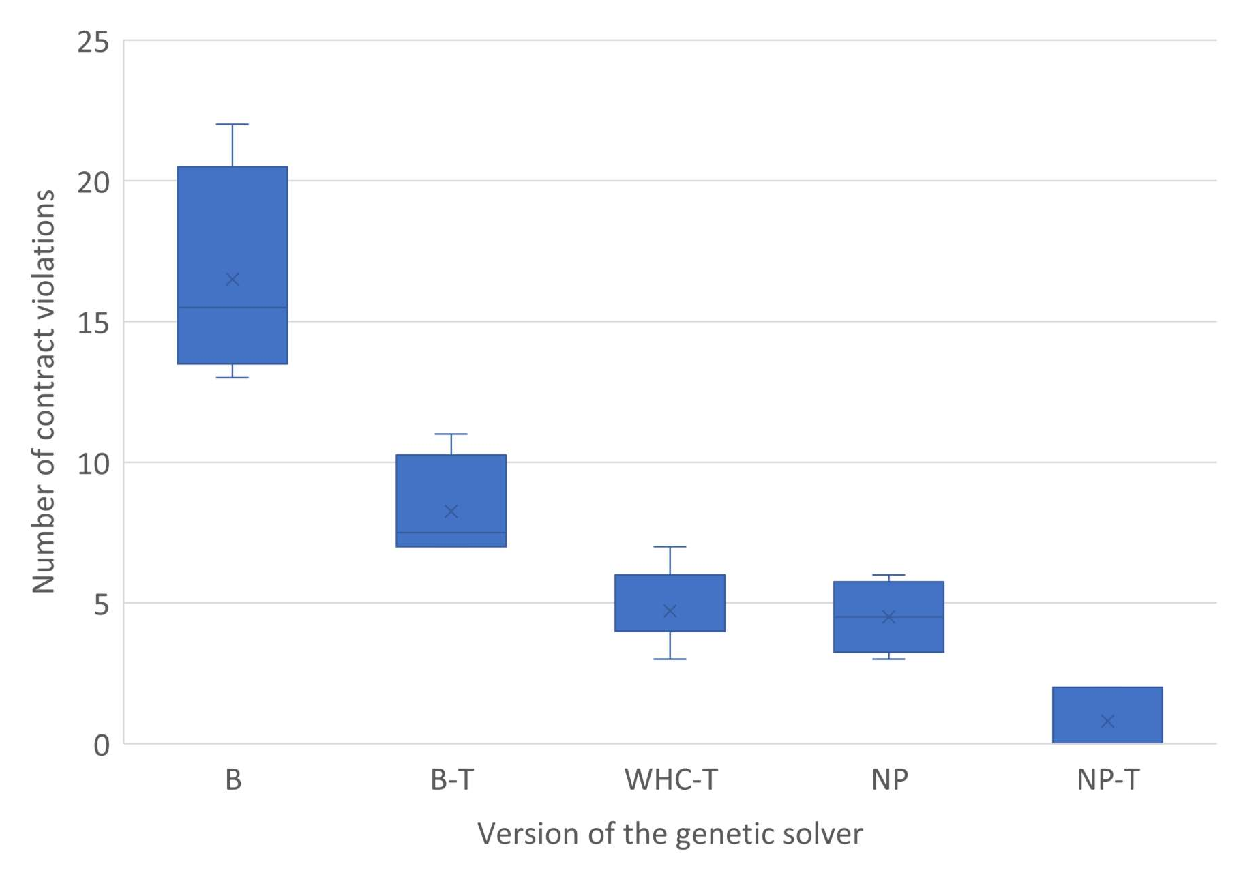
\includegraphics[width=\textwidth]{images/BoxPlotSolverNewParametersTuning.pdf}
	\caption[Boxplot with a number of contract violations for the genetic solver with added probabilities and tuned parameters in comparison with previous versions]{Boxplot with a number of contract violations for the genetic solver with added probabilities and tuned parameters in comparison with previous versions}
	\label{fig:boxplotsolverNewParametersTuning}
\end{figure}

Boxplots in Figure~\ref{fig:boxplotsolverNewParametersTuning} shows the comparisons of the NP-T version of the genetic solver to earlier discussed versions. As shown, the combined approach of parameter engendering and parameter tuning gives a zero number of contract violations. It means that the NP-T version has a \textbf{valid} solution for the MQuAT problem described at the beginning of this chapter. Even the worth-case of the NP-T version with two contract violations is better than all versions presented in previous sections.  

This section showed that the parameters thought out in the algorithm are as important as the values of these parameters. If the algorithm is not designed correctly, the tuning parameter may improve the results, but this may not be enough. It is worth noting that not all solutions of this version gave a valid solution. The reason for this is the local optimum. All versions of the genetic solver that were previously discussed cannot get out of the local optimum.  It could not get out because, at a certain moment, the majority of the individual in the population becomes the same.

\section{Simple parameter control parameters}

The reason all individuals become the same is due to the creation of offspring. To create new individuals, the selector takes the best individuals. Crossover, takes two individuals from the selector, and performing a gene change, creates two new individuals. If these individuals give a worse solution, then the selector in the new iteration will drop them, and if they are close, they will take them to create new individuals. At a certain point, it will be a situation that the crossover occurs between two identical genotypes, which creates two the same individuals. There is a chase \texttt{1~-~mutationRate} that mutation will not happen, and two identical as parents individuals will be added to the population. It increases the number of identical elements and leads to the collapse of the genetic diversity of the population.

The idea of how to solve this issue is internally changeable crossover rate. It changes the chance of the crossover depends on the number of the same individuals in a population. 
The principle of operation is as follows. After each iteration, a part of the unique genotypes in the population is calculated. If the resulting number is smaller than value of \texttt{PartOfUniqueIndividualsToStopCrossover} parameter, then the probability of a crossover will set as 0.0. And vice versa, the probability of a crossover returns back if the part of the unique genotypes in the population is bigger than value of \texttt{PartOfUniqueIndividualsToReturnCrossover} parameter.

The value for \texttt{PartOfUniqueIndividualsToStopCrossover} is 0.25 and for \texttt{PartOfUniqueIndividualsToReturnCrossover} is 0.75.

The version of the genetic solver with internally changeable crossover rate marked as \textbf{ICCR}(Internally Changeable Crossover Rate)~\footnote{commit: \href{https://git-st.inf.tu-dresden.de/mquat/mquat2/commit/c89422c6e46a5f4e8bc09205df7713ad8fe6907c}{c89422c6e46a5f4e8bc09205df7713ad8fe6907c}} and tuned version~\footnote{commit: \href{https://git-st.inf.tu-dresden.de/mquat/mquat2/commit/128a6f2f844edd70d0e8ee616f09ac897cb86f4e}{128a6f2f844edd70d0e8ee616f09ac897cb86f4e}} was marked as \textbf{ICCR-T}(Internally Changeable Crossover Rate-Tuned).

The parameter sets used for both versions presented in Table~\ref{tab:Parameters_ICCR-T}.

\begin{table}
	\centering
	\caption{Parameters of ICCR and ICCR-T versions of the genetic solver}\label{tab:Parameters_ICCR-T}
	\resizebox{\textwidth}{!}{
		\begin{tabular}{c c c c c c c c c c c c c c c c c c c}
			\hline
			\rotatebox{90}{Genetic solver} & 
			\rotatebox{90}{\texttt{selectorType}} & \rotatebox{90}{\texttt{PopulationSize}} & 
			\rotatebox{90}{\texttt{lambda}} & 
			\rotatebox{90}{\texttt{CrossoverRate}} & 
			\rotatebox{90}{\texttt{mu}} & 
			\rotatebox{90}{\texttt{MutationRate}} & \rotatebox{90}{\texttt{ResourceMutationProbability}}  & \rotatebox{90}{\texttt{ValidityWeight}} & \rotatebox{90}{\texttt{SoftwareValidityWeight}} & \rotatebox{90}{\texttt{RandomSoftwareAssignmentAttempts}} & \rotatebox{90}{\texttt{populateSoftwareSolutionAttempts}} &
			\rotatebox{90}{\texttt{CrossoverOnRandomChildProbability}} &
			\rotatebox{90}{\texttt{CrossoverOnRandomLevelProbability}} &
			\rotatebox{90}{\texttt{CrossoverOnRandomRequestProbability}} &
			\rotatebox{90}{\texttt{MutationOnRandomChildProbability}} &
			\rotatebox{90}{\texttt{MutationOnRandomLevelProbability}} &
			\rotatebox{90}{\texttt{PartOfUniqueIndividualsToStopCrossover}} &
			\rotatebox{90}{\texttt{PartOfUniqueIndividualsToReturnCrossover}} \\
			\hline			
			ICCR & NSGA2 & 500 & 0.1 & 0.95 & 0.1 & 0.45 & 0.5 & 0.5 & 0.5 & 50 & 100 & 0.5 & 0.5 & 0.0 & 0.5 & 0.5 & 0.25 & 0.75 \\
			ICCR-T & SPEA2 & 2550 & 0.5 & 0.5 & 0.5 & 0.5 & 0.5 & 0.5 & 0.5 & 500 & 500 & 0.5 & 0.5 & 0.5 & 0.5 & 0.5 \\
			\hline
		\end{tabular}
	}
\end{table}


\begin{figure}
	\centering
	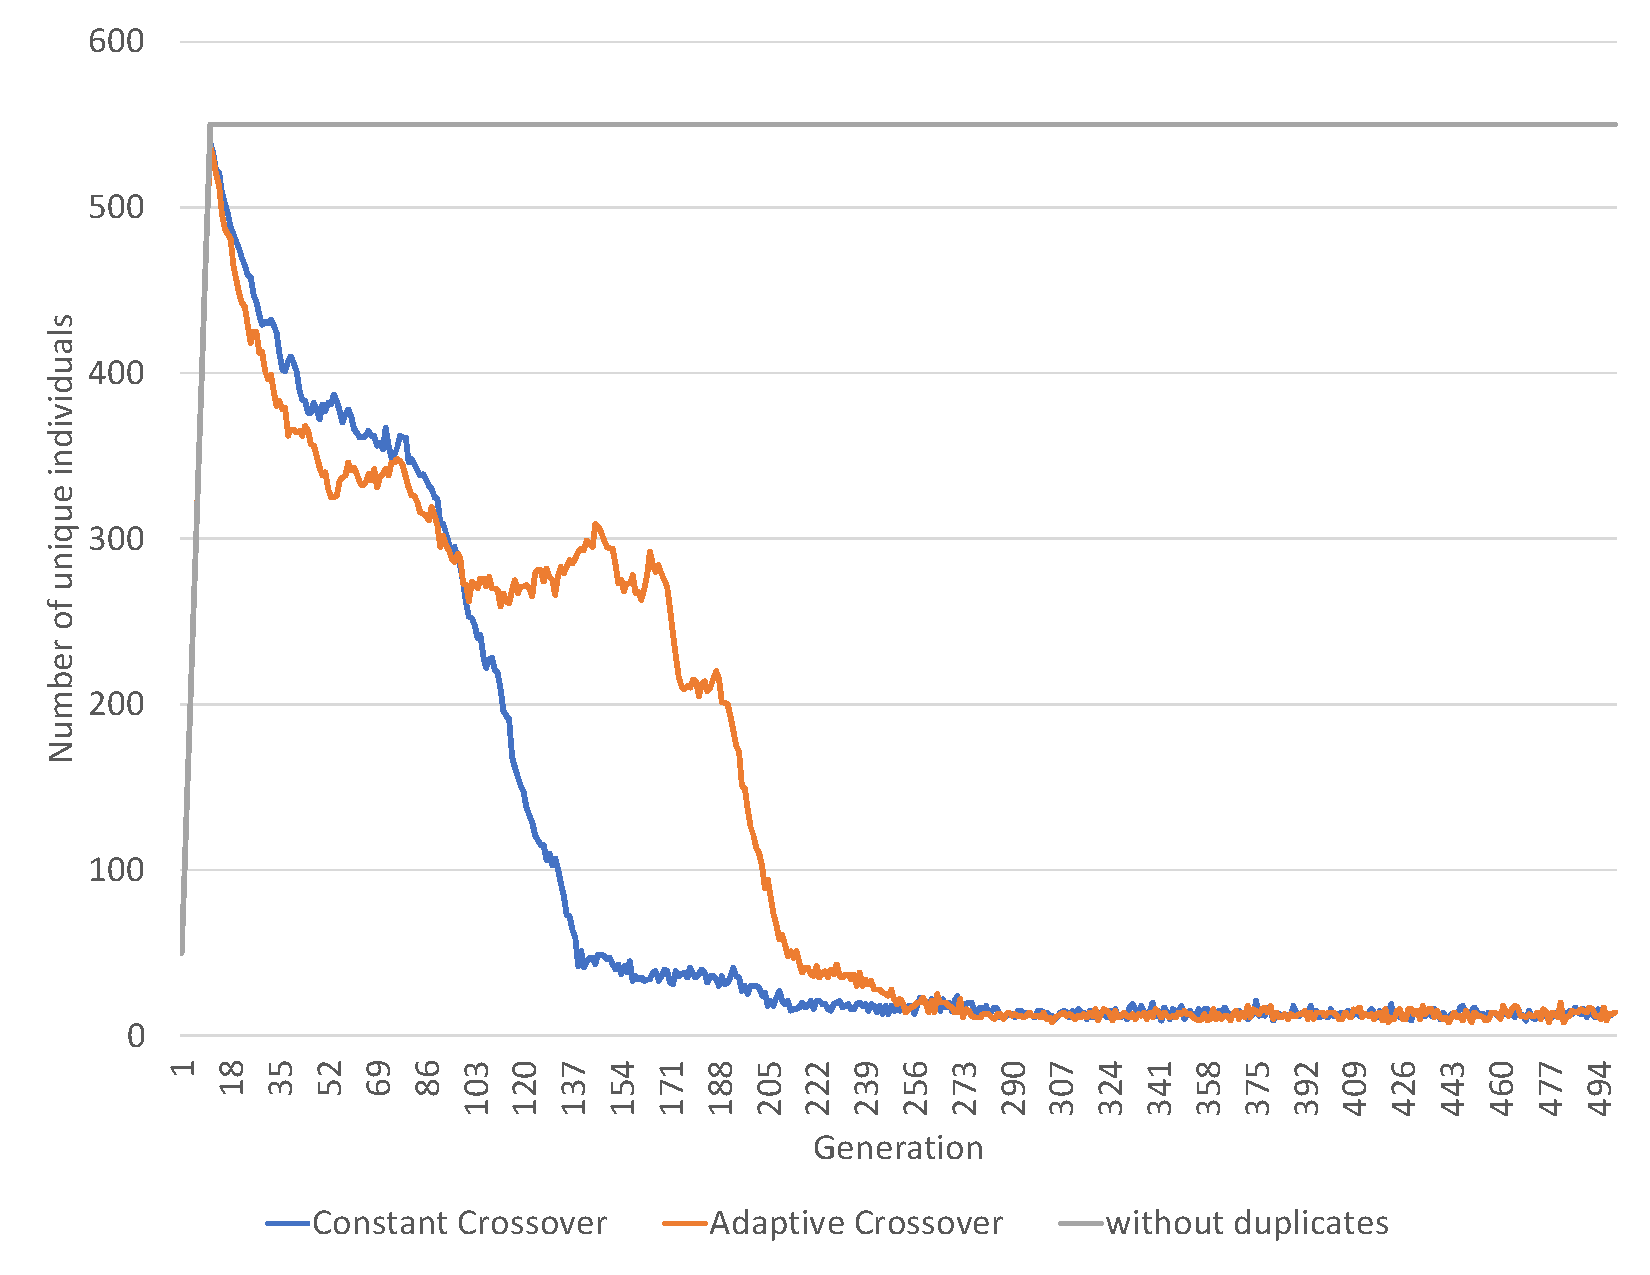
\includegraphics[width=\textwidth]{images/UniqIndividualsPerGeneration3.pdf}
	\caption[]{}
	\label{fig:UniqIndividualsPerGeneration3}
\end{figure} 


The internally changeable crossover rate slightly delay the collapse of the diversity of individuals in the population. Figure~\ref{fig:UniqIndividualsPerGeneration3} shows the deterioration in population diversity for a constant crossover rate and an internally changeable crossover rate.


The comparison of the results of ICCR and ICCR-T versions with all earlier discussed versions presented as boxplots showed in Figure~\ref{fig:boxplotsolverAdaptiveCrossoverTuning}. The ICCR version gives a better results than all untuned versions of the genetic solver. But the range between max and min number of contract violations in the ICCR version is bigger than in the NP version.
The ICCR also better the tuned versions such as B-T and WHC-T, but worse than the NP-T version. The ICCR-T version as a NP-T version gives a valid solution, but it is more like exception. The boxplot of ICCR-T version also shows that parameter tuning for internally changeable parameters works not so efficient as for static parameters like in NP version, at least for the discussed problem. 

\begin{figure}
	\centering
	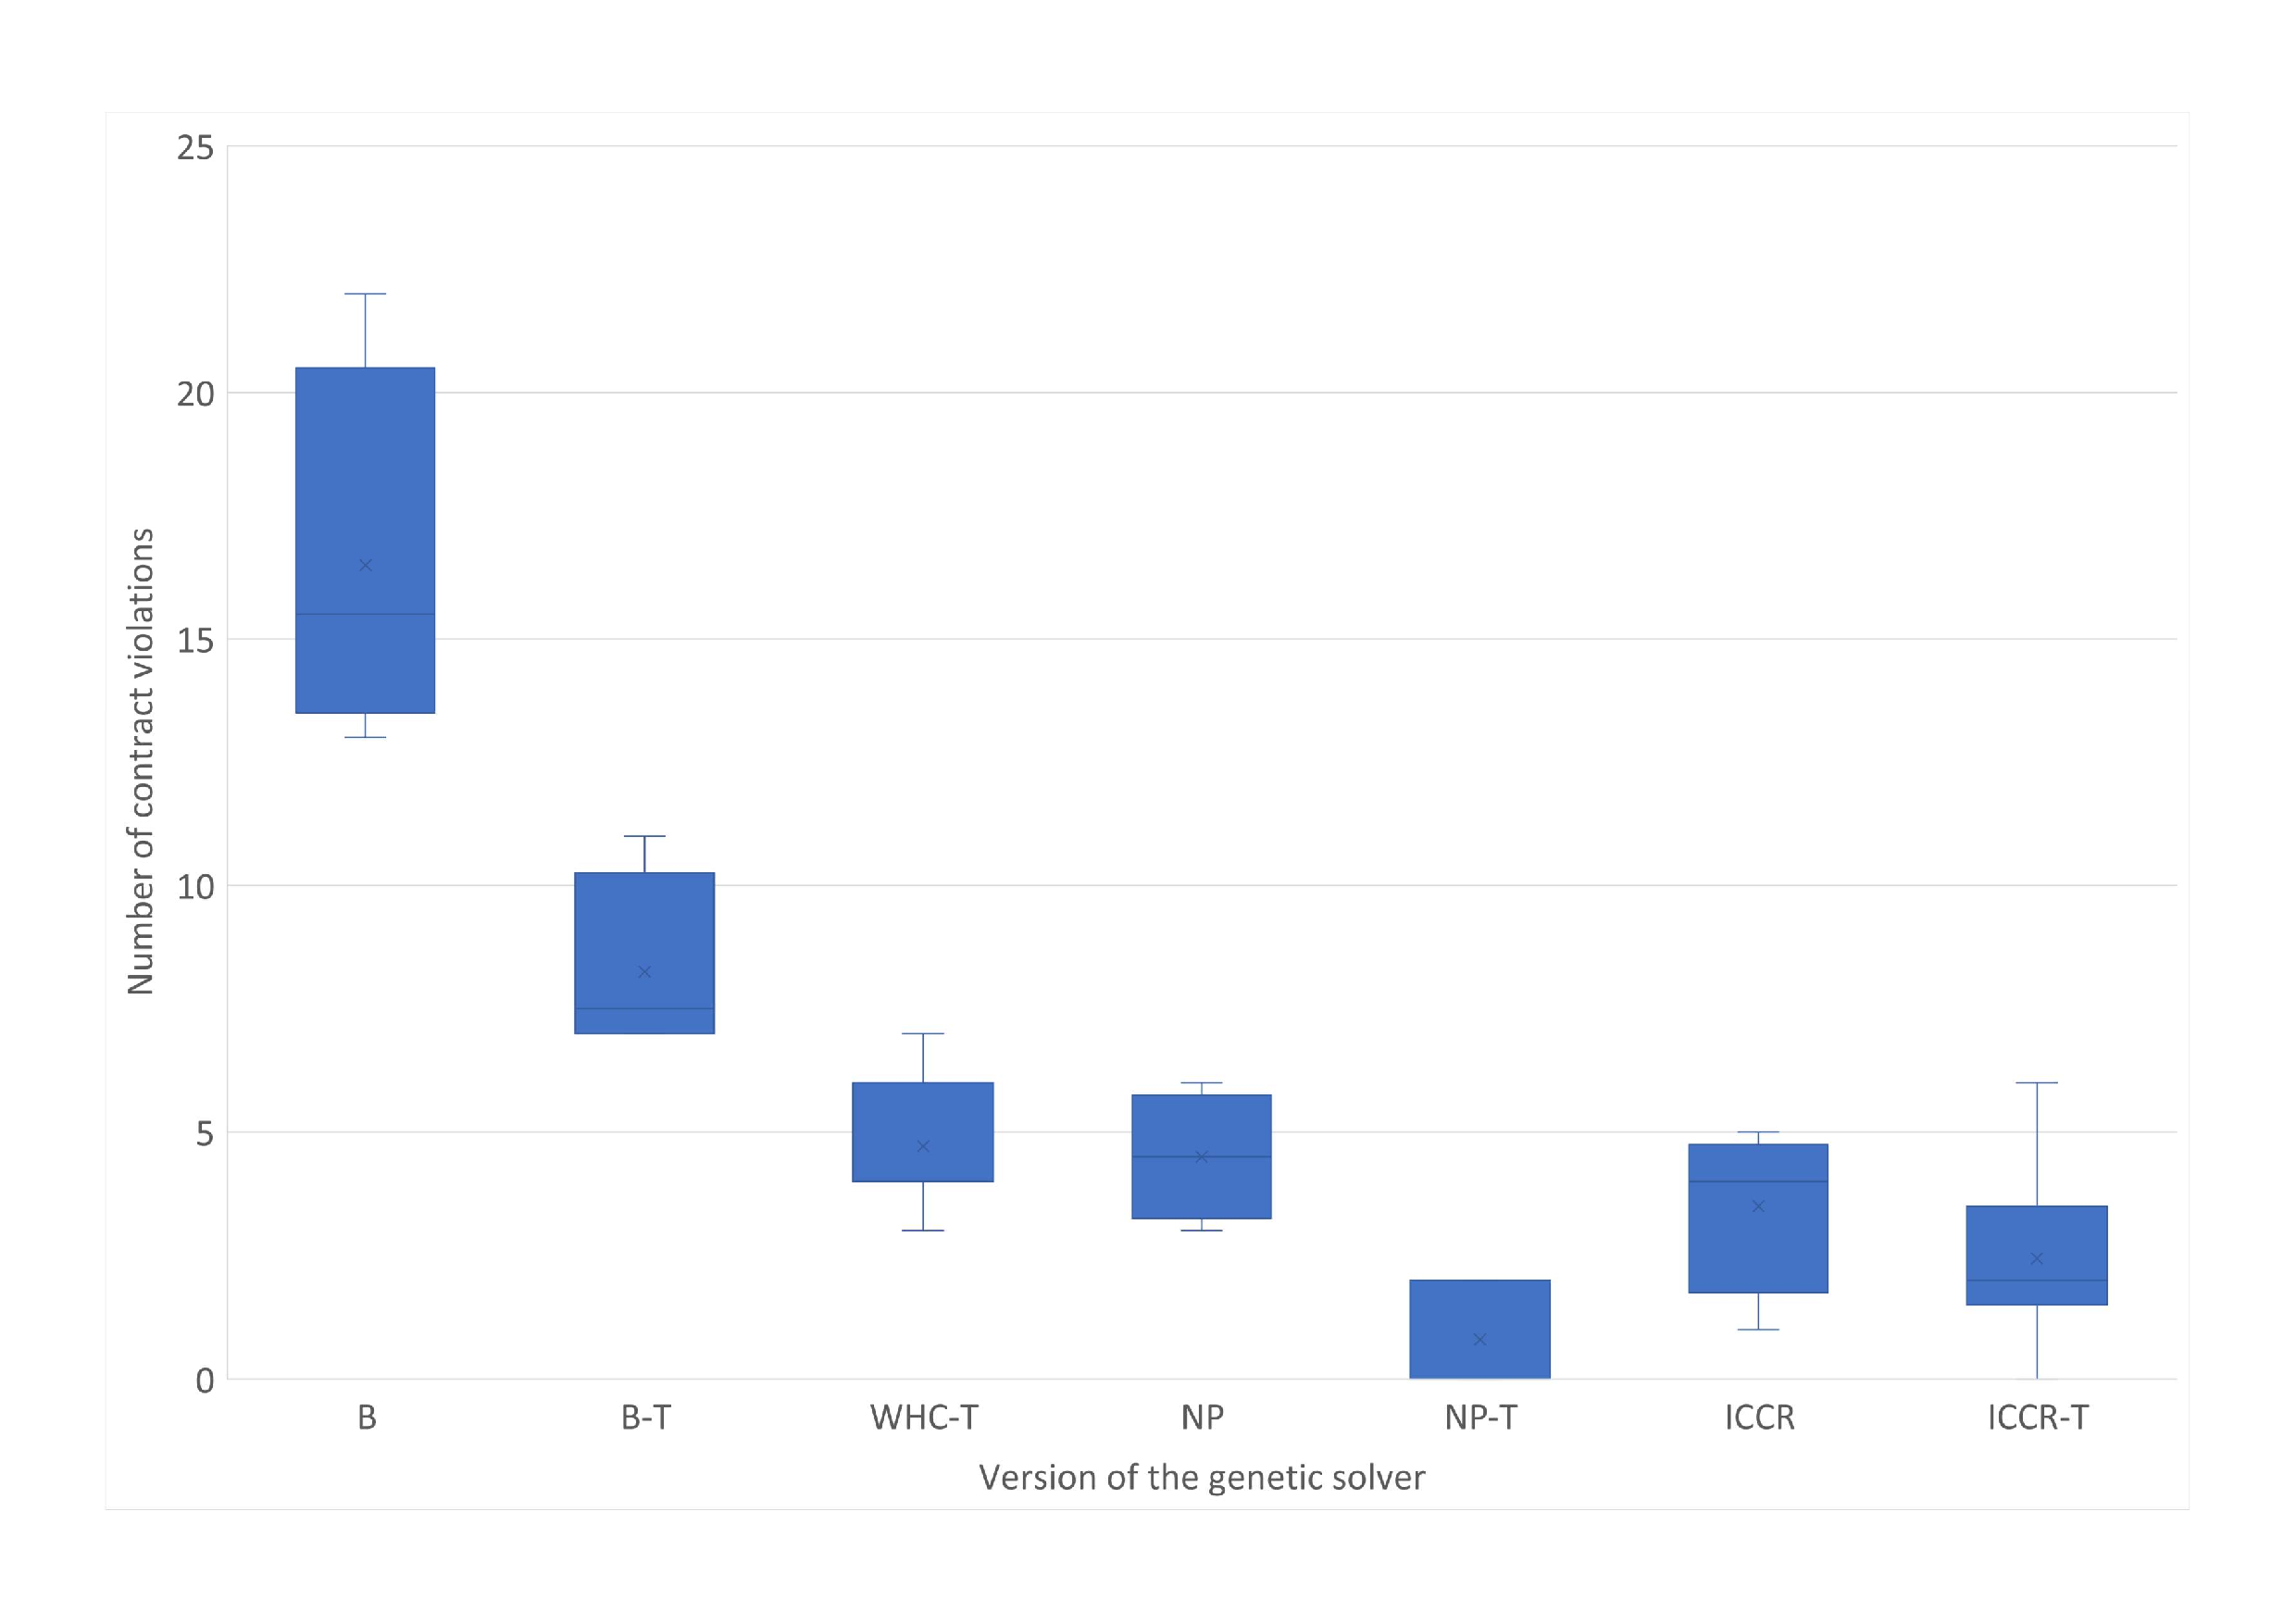
\includegraphics[width=\textwidth]{images/BoxPlotSolverAdaptiveCrossoverTuning.pdf}
	\caption[Boxplot with a number of contract violations for the genetic solver with adaptive crossover rate in comparison with previous versions]{Boxplot with a number of contract violations for the genetic solver with adaptive crossover rate in comparison with previous versions}
	\label{fig:boxplotsolverAdaptiveCrossoverTuning}
\end{figure}


This section shows that parameter control could improve the results and delay stuck in a local optimum. However, parameter tuning for static parameters does not work so well on parameters that changing their values during the work.                     

\section{Unique genotypes in a population}
\label{sec:WD}

Because the changeable crossover rate from the previous section only delays the collapse of the diversity of individuals in the population. We decide to try a more radical solution. We block the possibility of adding to the population a new individual if the population already contains the same individual. It means that at any moment, the population will consist of unique individuals. In this version of the genetic solver, the use of the changeable crossover rate does not make any sense, so it was disabled, and a constant value was used.

The number of unique individuals in the population for the WD version presented in Figure~\ref{fig:UniqIndividualsPerGeneration3}. On each generation after initial population have been created, the number of unique elements in population is not changing.

Untuned version ot the genetic solver with blocked duplicates in the population marked as  \textbf{WD}~\footnote{commit: \href{https://git-st.inf.tu-dresden.de/mquat/mquat2/commit/1d79c50d7932c9216c653bf6d0354d990f6aecbc}{1d79c50d7932c9216c653bf6d0354d990f6aecbc}}~(Without Duplicates)and tuned version~\footnote{commit: \href{https://git-st.inf.tu-dresden.de/mquat/mquat2/commit/24504c77024ac383c77849c5121471e0f06ce913}{24504c77024ac383c77849c5121471e0f06ce913}} marked as \textbf{WD-T}~(Without Duplicates-Tuned).

Parameters for both versions presented in Table~\ref{tab:Parameters_WD-T}.


\begin{table}
	\centering
	\caption{Parameters of WD and WD-T versions of the genetic solver}\label{tab:Parameters_WD-T}
	\resizebox{\textwidth}{!}{
		\begin{tabular}{c c c c c c c c c c c c c c c c c}
			\hline
			\rotatebox{90}{Genetic solver} & 
			\rotatebox{90}{\texttt{selectorType}} & \rotatebox{90}{\texttt{PopulationSize}} & 
			\rotatebox{90}{\texttt{lambda}} & 
			\rotatebox{90}{\texttt{CrossoverRate}} & 
			\rotatebox{90}{\texttt{mu}} & 
			\rotatebox{90}{\texttt{MutationRate}} & \rotatebox{90}{\texttt{ResourceMutationProbability}}  & \rotatebox{90}{\texttt{ValidityWeight}} & \rotatebox{90}{\texttt{SoftwareValidityWeight}} & \rotatebox{90}{\texttt{RandomSoftwareAssignmentAttempts}} & \rotatebox{90}{\texttt{populateSoftwareSolutionAttempts}} &
			\rotatebox{90}{\texttt{CrossoverOnRandomChildProbability}} &
			\rotatebox{90}{\texttt{CrossoverOnRandomLevelProbability}} &
			\rotatebox{90}{\texttt{CrossoverOnRandomRequestProbability}} &
			\rotatebox{90}{\texttt{MutationOnRandomChildProbability}} &
			\rotatebox{90}{\texttt{MutationOnRandomLevelProbability}} \\
			\hline			
			WD & NSGA2 & 500 & 0.1 & 0.95 & 0.1 & 0.45 & 0.5 & 0.5 & 0.5 & 50 & 100 & 0.5 & 0.5 & 0.0 & 0.5 & 0.5 \\
			WD-T & SPEA2 & 1057 & 0.49 & 0.66 & 0.82 & 0.04 & 0.95 & 0.09 & 0.04 & 929 & 383 & 0.68 & 0.85 & 0.51 & 0.41 & 0.65 \\
			\hline
		\end{tabular}
	}
\end{table}

\begin{figure}
	\centering
	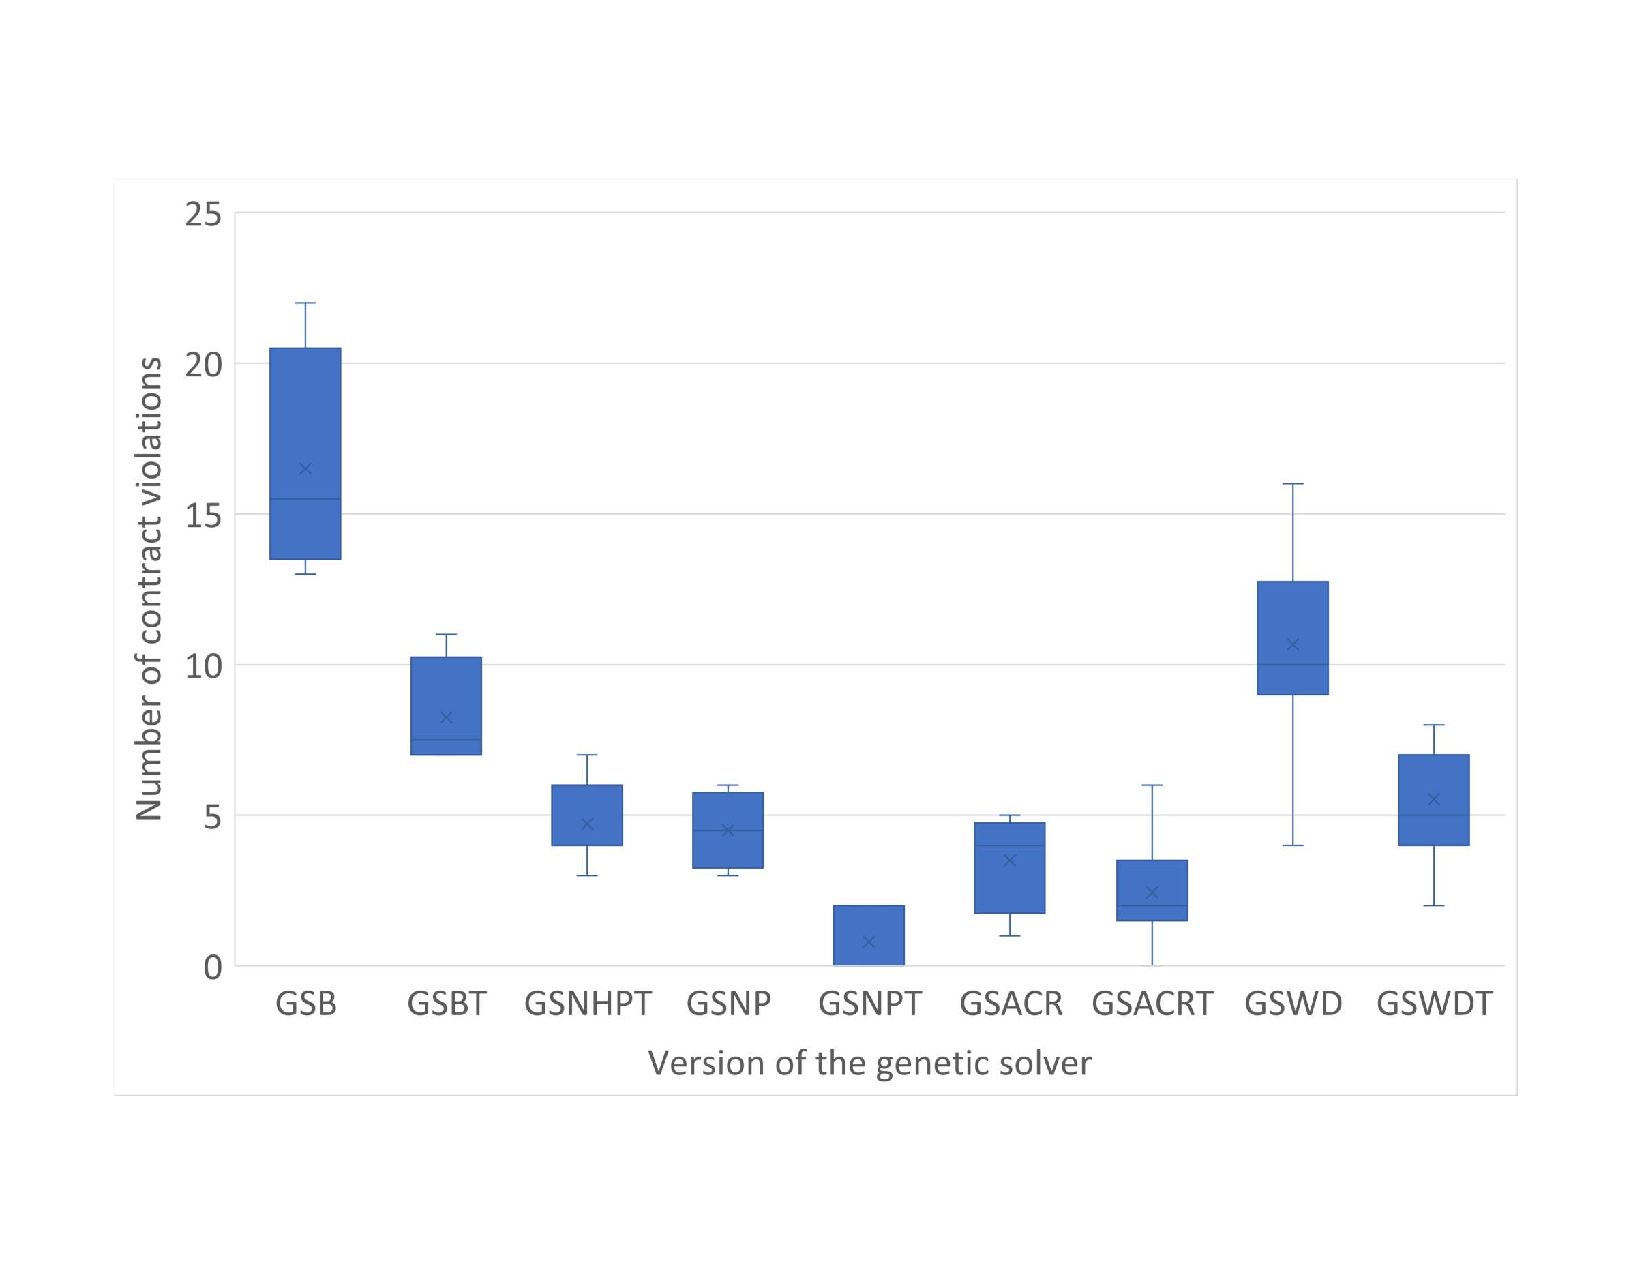
\includegraphics[width=\textwidth]{images/BoxPlotSolverNoDuplicates.pdf}
	\caption[Boxplot with a number of contract violations for the genetic solver without duplicates in the population in comparison with previous versions]{Boxplot with a number of contract violations for the genetic solver without duplicates in the population in comparison with previous versions}
	\label{fig:boxplotsolverNoDuplicates}
\end{figure} 

Figure~\ref{fig:boxplotsolverNoDuplicates} shows the results of this approach without tuning and with tuned parameters. Presented results show that the WD version of the genetic solver gives better results only in comparison to the B version and not always. The WD-T version gives better results with less range between min and max number of contract violations than WD. But it much worse than NP-T.

There are two main reasons why the results of this approach are much worse than previous versions. The first one is a calculation speed. It is slower than in previous versions. As a result, the number of created generations is lower. For the NP version, this number is 15177. For the WD version, this number is 2605, more than five times less according to our tests.

The second reason is a small number of "good" individuals selected to create offspring. This number is low because the selector could select the best individual from the population only once per selection. As a result, selected the best individual could give a few new individuals. Theoretically, the small value of the \texttt{mu} parameter could help. Nevertheless, BRISE gives the value of the \texttt{mu} parameter even higher than the default value. 

The conclusion of this idea is quite pessimistic because other approaches work better on this problem, but it may work better than others with different problems or on long term optimization.


\begin{table}
	\centering
	\caption{Parameters of NP and NP-T versions of the genetic solver}\label{tab:Parameters_all_versions}
	\resizebox{\textwidth}{!}{
		\begin{tabular}{c c c c c c c c c c c c c c c c c c c c}
			\hline
			\rotatebox{90}{Genetic solver} & 
			\rotatebox{90}{\texttt{selectorType}} & \rotatebox{90}{\texttt{PopulationSize}} & 
			\rotatebox{90}{\texttt{lambda}} & 
			\rotatebox{90}{\texttt{CrossoverRate}} & 
			\rotatebox{90}{\texttt{mu}} & 
			\rotatebox{90}{\texttt{MutationRate}} & \rotatebox{90}{\texttt{ResourceMutationProbability}}  &
			\rotatebox{90}{\texttt{crossoverProbability}}  & \rotatebox{90}{\texttt{ValidityWeight}} & \rotatebox{90}{\texttt{SoftwareValidityWeight}} & \rotatebox{90}{\texttt{RandomSoftwareAssignmentAttempts}} & \rotatebox{90}{\texttt{populateSoftwareSolutionAttempts}} &
			\rotatebox{90}{\texttt{CrossoverOnRandomChildProbability}} &
			\rotatebox{90}{\texttt{CrossoverOnRandomLevelProbability}} &
			\rotatebox{90}{\texttt{CrossoverOnRandomRequestProbability}} &
			\rotatebox{90}{\texttt{MutationOnRandomChildProbability}} &
			\rotatebox{90}{\texttt{MutationOnRandomLevelProbability}} &
			\rotatebox{90}{\texttt{PartOfUniqueIndividualsToStopCrossover}} &
			\rotatebox{90}{\texttt{PartOfUniqueIndividualsToReturnCrossover}} \\
			\hline			
			B & NSGA2 & 500 & \cellcolor{Gray} 0.1 & \cellcolor{Gray} 0.95 & \cellcolor{Gray} 0.1 & \cellcolor{Gray} 0.45 & \cellcolor{Gray} 0.5 & \cellcolor{Gray} 0.8 & \cellcolor{Gray} 0.5 & \cellcolor{Gray} 0.5 & \cellcolor{Gray} 50 & \cellcolor{Gray} 100 \\
			
			B-T & NSGA2 & 1533 & \cellcolor{Gray} 0.1 & \cellcolor{Gray} 0.95 & \cellcolor{Gray} 0.1 & \cellcolor{Gray} 0.45 & \cellcolor{Gray} 0.5 & \cellcolor{Gray} 0.8 & \cellcolor{Gray} 0.5 & \cellcolor{Gray} 0.5 & \cellcolor{Gray} 50 & \cellcolor{Gray} 100 \\	
					
			WHC-T & SPEA2 & 2014 & 0.98 & 0.95 & 0.58 & 0.02 & 0.64 & 0.3 & 0.95 & 0.17 & 79 & 266 \\
						
			NP & NSGA2 & 500 & 0.1 & 0.95 & 0.1 & 0.45 & 0.5 & & 0.5 & 0.5 & 50 & 100 & 0.5 & 0.5 & 0.0 & 0.5 & 0.5 \\
			
			NP-T & NSGA2 & 2550 & 0.5 & 0.5 & 0.5 & 0.5 & 0.5 & & 0.5 & 0.5 & 500 & 500 & 0.5 & 0.5 & 0.5 & 0.5 & 0.5 \\
						
			ICCR & NSGA2 & 500 & 0.1 & 0.95 & 0.1 & 0.45 & 0.5 & 0.5 & 0.5 & 50 & 100 & 0.5 & 0.5 & 0.0 & 0.5 & 0.5 & 0.25 & 0.75 \\
			
			ICCR-T & SPEA2 & 2550 & 0.5 & 0.5 & 0.5 & 0.5 & 0.5 & 0.5 & 0.5 & 500 & 500 & 0.5 & 0.5 & 0.5 & 0.5 & 0.5 \\
					
			WD & NSGA2 & 500 & 0.1 & 0.95 & 0.1 & 0.45 & 0.5 & & 0.5 & 0.5 & 50 & 100 & 0.5 & 0.5 & 0.0 & 0.5 & 0.5 \\
			
			WD-T & SPEA2 & 1057 & 0.49 & 0.66 & 0.82 & 0.04 & 0.95 & & 0.09 & 0.04 & 929 & 383 & 0.68 & 0.85 & 0.51 & 0.41 & 0.65 \\
			\hline
		\end{tabular}
	}
\end{table}
\todoR{Do I really need this table?}


